\documentclass[10pt,letterpaper]{book}
\usepackage[utf8]{inputenc}
\usepackage[spanish]{babel}
\usepackage[top=3cm,bottom=5cm,left=4cm,right=4cm]{geometry}
\usepackage[colorlinks, linkcolor=black, citecolor=magenta]{hyperref}
\usepackage{cleveref}
\usepackage{graphicx}
\usepackage[svgnames]{xcolor}
\usepackage{minted}
\usemintedstyle{pastie}
\setminted{bgcolor=WhiteSmoke, breaklines}
\AtEndEnvironment{listing}{\vspace{-1em}} % stretch listing's caption distance
\usepackage{emptypage}
\usepackage{caption}

\usepackage[dotinlabels]{titletoc}
\titlecontents
{chapter}
[1.5pc]
{\addvspace{1pc}\bfseries\titlerule[1pt]\filright\addvspace{0.3pc}}
{\contentslabel[\thecontentslabel]{1.5pc}}
{}
{\hfill\contentspage}
[\addvspace{2pt}]

\usepackage[Rejne]{fncychap}
\makeatletter
\renewcommand{\DOCH}{
    \settoheight{\py}{\CNoV\thechapter}
    \parskip=0pt plus 20pt
    \addtolength{\py}{-1pt}
    \CNV
\includegraphics[scale=0.5]{images/coffee_beans.png}\par\nobreak
    \vskip 20\p@
    \setlength{\myhi}{2\baselineskip}
    \setlength{\px}{\myhi}
    \addtolength{\px}{-1\RW}
    \rule[-1\px]{\RW}{\myhi}\mghrulefill{\RW}\hskip 10pt
    \raisebox{-0.5\py}{\CNoV\thechapter}\hskip 10pt
    \mghrulefill{\RW}\rule[-1\px]{\RW}{\myhi}\par\nobreak
    \vskip -5\p@
    }
    \makeatother

\usepackage{fancyhdr}
\pagestyle{fancy}
\setlength\headheight{50pt}
\lhead{
\includegraphics[scale=0.1]{images/coffee_beans.png}}
\fancyhead[LE,RO]{
\includegraphics[scale=0.1]{images/coffee_beans.png}}
\fancyhead[RE,LO]{\rightmark}

\renewcommand\listoflistingscaption{Índice de códigos}
\renewcommand\listingscaption{Código}
\crefname{listing}{código}{códigos}
\Crefname{listing}{Código}{Códigos}
\crefname{table}{tabla}{tablas}
\Crefname{table}{Tabla}{Tablas}
\crefname{figure}{figura}{figuras}
\Crefname{figure}{Figura}{Figuras}
\crefname{section}{sección}{secciones}
\Crefname{section}{Sección}{Secciones}

\title{

\includegraphics[scale=0.7]{images/coffee_beans.png} \\\vspace{2em}
Clasificación de hojas de café infectadas por roya usando segmentación por matices en el canal Hue}
\author{Línderman Emmanuel Domínguez Ordóñez}
\date{Agosto de 2025}
\begin{document}
\renewcommand{\listtablename}{Índice de tablas}
\renewcommand{\tablename}{Tabla}
\maketitle
\frontmatter
\pagestyle{plain}
\tableofcontents
\listoflistings
\listoffigures
\listoftables
\mainmatter
\pagestyle{fancy}
\chapter{Introducción}

\section{Procesamiento Digital de Imágenes}
Una imagen digital puede considerarse como una función 2-dimensional que representa puntos en el espacio llamados pixeles los cuales son finitos y discretos, y que presentan una intensidad definida. El \textit{Procesamiento Digital de Imágenes} hace referencia al proceso de manipular imágenes digitales mediante el uso de computadoras.

La visión es nuestro sentido más avanzado, sin embargo, estamos limitados a las capacidades biológicas de nuestros ojos para la percepción de imágenes. Una computadora en cambio tiene la facilidad de poder adaptar su espectro visual más allá de lo que nosotros somos capaces de ver.

No existe una frontera bien definida sobre dónde el procesamiento de imágenes termina respecto a otras áreas como el análisis de imágenes y la visión por computadora. Sin embargo, podemos considerar tres tipos de procesos computarizados que determinan el nivel de procesamiento llevado acabo.

Los procesos de bajo nivel que involucran operaciones primitivas tales como la reducción de ruido o la mejora del contraste. Estos procesos reciben como entrada una imagen y producen como salida otra imagen. Los procesos de nivel intermedio, que usualmente reciben una imagen de entrada pero que producen como salida los atributos o características de la imagen proporcionada, tales como bordes, contornos, etc. Y finalmente los procesos de alto nivel que buscan darle sentido a las imágenes procesadas aplicando funciones congnitivas generalmente asociadas a la visión.

En general, el \textit{Procesamiento Digital de Imágenes} involucra los procesos que reciben y generan imágenes y que opcionalmente pueden extraer sus características. \cite{gonzalez2008digital}

\section{Procesamiento Digital de Imágenes: Fundamentos y Aplicaciones con GNU Octave y OpenCV}
Durante los meses de junio a agosto de 2025 se impartió el seminario \textit{Procesamiento Digital de Imágenes: Fundamentos y Aplicaciones con GNU Octave y OpenCV} a través de la \textit{Benemérita Universidad Autónoma de Chiapas} y dicatado por el \textit{PhD. Luis Escalante Zárate} en el cual se revisaron los conceptos y métodos tradicionales del procesamiento digital de imágenes tales como filtros, segmentación, creación de máscaras, histogramas, espacios de color, transformaciones en el dominio de la frecuencia, etc. de manera práctica e intuitiva en sesiones diarias de seis horas por un total de seis semanas y dos más de revisiones personalizadas.

Las herramientas utilizadas en el curso fueron muy variadas como \textit{IrfanView} para la visualización y edición rápida de imágenes, \textit{Python} con \textit{OpenCV} para prueba de conceptos de manera agilizada, y destacando sobre todos el uso de \textit{GNU Octave} como una alternativa \textit{open-source} a la herramienta de \textit{MatLab}.

A partir de este seminario surge la necesidad del desarrollo de un proyecto que exponga el conocimiento adquirido y que sirva como memoria del curso.
\chapter{Planteamiento del problema}
El café es un producto altamente consumido en el mundo y es una de las bebidas más populares y preferidas en la sociedad. La producción de café representa un sustento económico para muchas familias en México y más precisamente en Chiapas que es uno de los principales estados exportadores de este grano.

El precio del café tuvo un incremento en el último año, sin embargo, las plagas representan un riesgo para su producción. Algunas plagas como la roya, la araña roja o la broca, pueden causar perdidas severas tanto económicas como de materia prima que bien podrían minimizarse o incluso prevenirse mediante un monitoreo adecuado y regular de la plantación evitando medidas drásticas correctivas como la aplicación de químicos.

El monitoreo de los cultivos de café generalmente require de capacitación o asesoría técnica especializada que muchas veces es cara o inaccesible. El proyecto \textit{Clasificación de hojas de café infectadas por roya usando segmentación por matices en el canal Hue} busca ofrecer una alternativa para quienes apenas ingresan en el mundo del café o bien si no se cuenta con los recursos de inversión suficientes.

\section{Objetivo general}
Demostrar las habilidades adquiridas durante el seminario \textit{Procesamiento Digital de Imágenes: Fundamentos y Aplicaciones con GNU Octave y Open CV} aplicando los principios y técnicas básicas de manera práctica a un proyecto en particular.

\section{Objetivo específico}
Crear un algoritmo que clasifique hojas de café como sanas o infectadas por roya y su nivel de afectación, y evaluar su eficiencia comparando los resultados obtenidos con los proporcionados en el conjunto de datos.

\section{Alcance}
A pesar de que el conjunto de datos de prueba contiene seis clasificaciones para las hojas, el algoritmo desarrollado sólo incluirá la clasificación sana y los cuatro niveles de afectación por roya, excluyendo la clasificación \textit{araña roja} debido a las retricciones en el tiempo del proyecto.

\section{Justificación}
El algoritmo y las técnicas utilizadas pueden aplicarse de manera directa en el mundo real dentro del área de la agricultura y/o agronomía, e idealmente puede servir como base para desarollar procesos automatizados para el control de calidad en el ámbito del café y control de plagas.
 
\section{Especificaciones técnicas}
Se utilizará \textit{Python} como lenguaje de programación para la implementación del algoritmo debido a su facilidad de uso y al amplio número de bibliotecas disponibles para el procesamiento de imágenes tales como \textit{OpenCV}. Así mismo, se utilizará una libreta de \textit{Jupyter} para la ejecución del algoritmo debido a su flexibilidad para ejecutar trozos de código de manera interactiva.

\section{Metodología}
El proceso comienza con la adquisición de las imágenes de las hojas de café, las cuales se transformarán del modelo RGB (Red, Green, Blue) al HSV (Hue, Saturation, Value) para poder aislar el canal Hue. Aplicando diferentes umbrales para los matices, segmentaremos la región de interés en busca de presencia de roya. Usando la imagen segmentada clasificaremos la severidad de la afectación a través de una operación entre el área de la imagen segmentada y una máscara que represente el área de la hoja. Finalmente revisaremos la eficiencia del algoritmo comparando nuestros resultados con las clasificaciones hechas por expertos.

\subsection{Modelo de color HSV}
El modelo de color HSV (Hue, Saturation, Value - Matiz, Saturación, Valor), también conocido como HSB (Hue, Saturation, Brightness - Matiz, Saturación, Brillo) es una representación no-lineal de los colores RGB (Red, Green, Blue - Rojo, Verde, Azul) que ofrece una representación más intuitiva ya que se asemeja a la forma en la que el ojo humano percibe el color.

\begin{figure}[H]
\centering
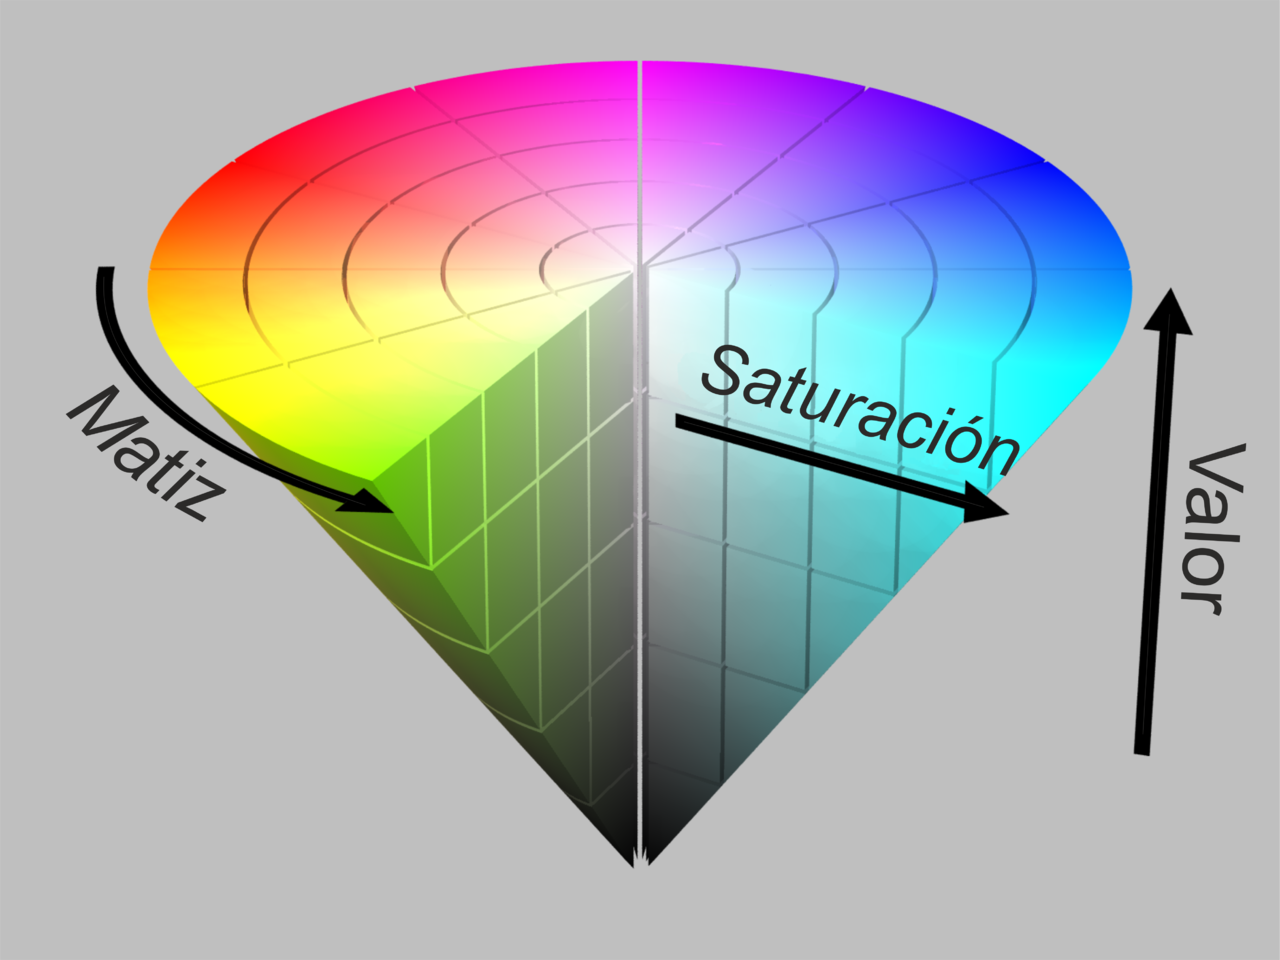
\includegraphics[scale=0.8]{images/hsv_model.png}
\caption{Modelo de color HSV}
\label{img:polygon}
\end{figure}

Una de sus principales ventajas en el ámbito del procesamiento digital de imágenes es que facilita la segmentación de objetos coloridos. Además que, en muchos contextos, el color está asociado a ciertas características inherentes del sistema bajo estudio.

Tal es el caso de la infección por roya en hojas de café, la cual produce cambios de color en las hojas afectadas e incluso cada color indicando un nivel de afectación diferente.

\subsection{RoCoLe: A robusta coffee leaf images dataset}
En el artículo \textit{RoCoLe: A robusta coffee leaf images dataset for evaluation of machine learning based methods in plant diseases recognition} \cite{PARRAGAALAVA2019104414}, Jorge Parraga-Alava, Kevin Cusme, Angélica Loor y Esneider Santander nos proporcionan el dataset \textit{RoCoLe: A robusta coffee leaf images dataset} \cite{RoCoLe} el cual contiene imágenes de hojas de café robusta manualmente clasificadas por su estado de salud y severidad de afectación por roya. Usaremos este dataset como la fuente de imágenes para nuestro proyecto y a su vez nos servirá como referencia para la verificación del desempeño de nuestro algoritmo.

\textit{RoCoLe} continene la información de 390 plantas de café robusta a las cuales se le tomaron 4 muestras de sus hojas haciendo un total de 1560 imágenes. Las muestras fueron tomadas en diferentes condiciones (iluminación, lado de la hoja) para proporcionar un conjunto más diverso de características.

Cada hoja presenta dos clasificaciones: la primera respecto a su estado de salud, ya sea saludable o no-saludable, y la segunda respecto al nivel de afectación por roya en caso de ser una hoja no-saludable. La \Cref{table:rust_levels} presenta la ponderación utilizada para la clasificación de los niveles de afectación.

\begin{table}[H]
\centering
\begin{tabular}{|c|c|c|c|}
\hline 
\textbf{Nivel} & \textbf{Categoría} & \textbf{Descripción} & \textbf{Área afectada} \\
\hline
1 & rust\_level\_1 & Roya nivel 1 & 1 - 5 \% \\
\hline 
2 & rust\_level\_2 & Roya nivel 2 & 6 - 20 \% \\
\hline 
3 & rust\_level\_3 & Roya nivel 3 & 21 - 50 \% \\
\hline 
4 & rust\_level\_4 & Roya nivel 4 & $>$ 50 \% \\
\hline 
\end{tabular}
\caption{Niveles de afectación por roya}
\label{table:rust_levels}
\end{table}
\chapter{Procedimiento}
A continuación se describen los procesos del algoritmo que permiten solucionar el problema especificado. El código fuente está disponible de manera digital en la plataforma de GitHub \cite{LindermanDgz}.

\section{Lectura del dataset}
Se comienza leyendo el dataset que contiene información que ha sido etiquetada de manera manual por los autores del mismo. Este proceso se describe en \Cref{code:load_dataset}.

\begin{listing}[!ht]
\inputminted{python}{code_listings/load_dataset.py}
\caption{Cargar las anotaciones del dataset}
\label{code:load_dataset}
\end{listing}

Utilizando la biblioteca \texttt{json} de Python leémos el archivo \texttt{RoCoLE.json} (originalmente \texttt{Annotations/RoCoLE-json.json}). La variable \texttt{annotations} contiene la información necesaria para contruir nuestro conjunto de datos de prueba (véase \Cref{table:required_annotations}).

\begin{table}[h!]
\centering
\begin{tabular}{|l|l|}
\hline 
\textbf{Anotación} & \textbf{Descripción} \\ 
\hline 
ID & Identificador de la hoja \\ 
\hline 
Label.Leaf.0.state & Estado de la hoja como saludable o infectada \\ 
\hline 
Label.classification & Clasificación de la hoja o nivel de afectación \\ 
\hline 
Label.Leaf.0.geometry & Puntos (x,y) que determinan el contorno de la hoja \\ 
\hline 
\end{tabular}
\caption{Anotaciones del dataset}
\label{table:required_annotations}
\end{table}

\subsection{La clase CoffeeLeaf}
A continuación creamos una clase llamada \texttt{CoffeeLeaf} la cual se encarga de contener los datos proporcionados en las anotaciones y que representa a una hoja de café. Los atributos de esta clase pueden observarse en \Cref{code:coffee_leaf}.

\begin{listing}[!ht]
\inputminted{python}{code_listings/coffee_leaf.py}
\caption{La clase CoffeeLeaf}
\label{code:coffee_leaf}
\end{listing}

Una vez creada la clase \texttt{CoffeeLeaf} y leído los datos del dataset, procedemos a crear la lista \texttt{coffee\_leaves} utilizando los datos de la \Cref{table:required_annotations}, tal como se muestra en \Cref{code:coffee_leaves}. El directorio \texttt{../rocole\_photos/} contiene los archivos \texttt{.jepg} del dataset (\texttt{Annotations/RoCoLe-voc.tar.gz/export}).

\begin{listing}[!ht]
\inputminted{python}{code_listings/coffee_leaves.py}
\caption{Lista de objetos CoffeLeaf}
\label{code:coffee_leaves}
\end{listing}

\section{Procesado de la imagen}
Una vez creada la lista \texttt{coffee\_leaves} iniciamos el procesamiento de las imagénes a través de la función \texttt{process} (\Cref{code:process}) de la clase \texttt{CoffeeLeaf}. Véase \Cref{code:process_iteration}.

\begin{listing}[!ht]
\inputminted{python}{code_listings/process.py}
\caption{Función process del la clase CoffeeLeaf}
\label{code:process}
\end{listing}

\begin{listing}[!ht]
\inputminted{python}{code_listings/process_iteration.py}
\caption{Iniciar procesamiento de las imágenes}
\label{code:process_iteration}
\end{listing}

\subsection{Conversión de BGR a RGB}
Debido a que cuando creamos los objetos \texttt{CoffeeLeaf} el argumento \texttt{image\_bgr} pasa datos de una imagen en color \textsf{BGR} (Blue, Green, Red), que es la representación de color por defecto de \textit{OpenCV}, y ya que \textit{matplotlib}, la herramienta para la visualización de las imágenes, utiliza una representación \textsf{RGB} (Red, Green, Blue), una conversión de color es necesaria. Véase \Cref{code:bgr_to_rgb}.

\begin{listing}[!ht]
\inputminted{python}{code_listings/bgr_to_rgb.py}
\caption{Convertir imgen BGR a RGB}
\label{code:bgr_to_rgb}
\end{listing}

El resultado de esta conversión permite visualizar la imagen original (\Cref{img:original}).

\begin{figure}[!ht]
\centering
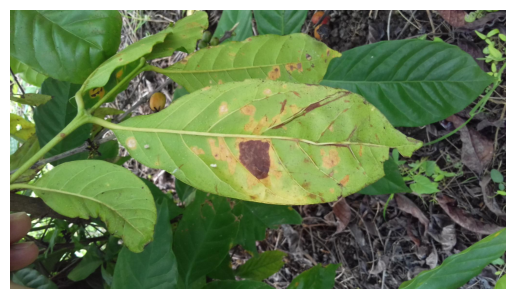
\includegraphics[scale=1]{images/original_image.png}
\caption{Imagen original en RGB}
\label{img:original}
\end{figure}

\subsection{Creación de las regiones de interés}
La anotación \texttt{geometry} del dataset nos provee de una serie de puntos \texttt{(x,y)} que representan el contorno de la hoja de café y que nos sirven para crear un polígono (\Cref{code:polygon}).

\begin{listing}[!ht]
\inputminted{python}{code_listings/polygon.py}
\caption{Puntos (x, y) del contorno de la hoja de café}
\label{code:polygon}
\end{listing}

El contorno de la hoja de café se puede apreciar en la \Cref{img:polygon}.

\begin{figure}[!ht]
\centering
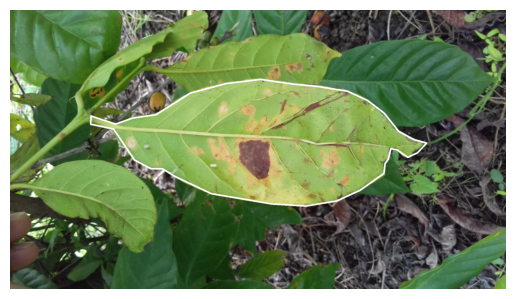
\includegraphics[scale=1]{images/polygon.png}
\caption{Polígono que delimita el contorno de la hoja}
\label{img:polygon}
\end{figure}

Posteriomente creamos el rectángulo mínimo que encierra a esta región, como se aprecia en la \Cref{img:bounding_rect} y lo usamos para recortar nuestra región de interés (véase \Cref{code:roi}).

\begin{figure}[!ht]
\centering
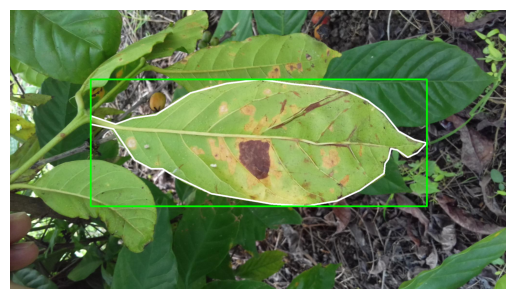
\includegraphics[scale=1]{images/bounding_rect.png}
\caption{Cuadro que aisla a la hoja de café}
\label{img:bounding_rect}
\end{figure}

\begin{listing}[!ht]
\inputminted{python}{code_listings/roi.py}
\caption{Crear regiones de interés}
\label{code:roi}
\end{listing}

Creamos dos regiones de interés: la primera en \textsf{RGB} (\Cref{img:roi_rgb}) para la presentación al usuario y la segunda en \textsf{HSV} (Hue, Saturation, Value) (\Cref{img:roi_hsv}) que nos servirá en la segmentación de la imagen.

\begin{figure}[!ht]
\centering
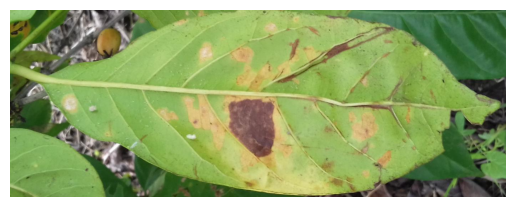
\includegraphics[scale=1]{images/roi_rgb.png}
\caption{Región de interés en RGB}
\label{img:roi_rgb}
\end{figure}

\begin{figure}[!ht]
\centering
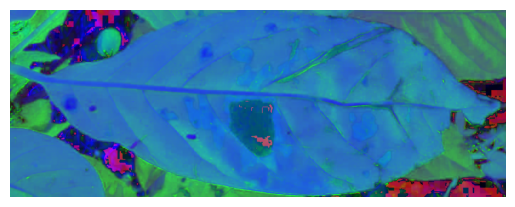
\includegraphics[scale=1]{images/roi_hsv.png}
\caption{Región de interés en HSV}
\label{img:roi_hsv}
\end{figure}

\subsection{Creación de la máscara}
Utilizando las regiones de interés previamente creadas y el polígono que delimita el contorno de la hoja, procedemos a crear una máscara (\Cref{code:mask}) que nos será útil en las operaciones matriciales del procesamiento de la imagen. Véase \Cref{img:mask}.

\begin{listing}[!ht]
\inputminted{python}{code_listings/mask.py}
\caption{Crear máscara}
\label{code:mask}
\end{listing}

\begin{figure}[!ht]
\centering
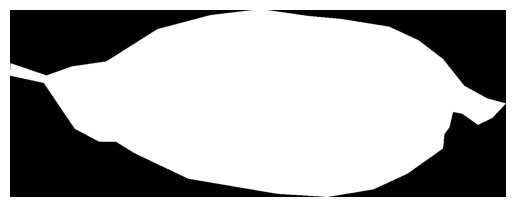
\includegraphics[scale=1]{images/mask.png}
\caption{Máscara}
\label{img:mask}
\end{figure}

Nótese que en \Cref{code:mask} calculamos el área que ocupa la máscara (pixeles en color blanco), o lo que es mismo, el área de la hoja de café.

\subsection{Enmascaramiento de las regiones de interés}
Una vez teniendo la máscara y las regiones de interés, procedemos a \textit{enmascarar} dichas regiones (\Cref{code:masked_roi}). Para el caso de la región de interés en \textsf{RGB} es por mera conveniencia al presentar esta región al usuario. Sin embargo, para el enmascaramiento de la region de interés en \textsf{HSV} es de suma importancia usar únicamente el canal Hue (Matiz) puesto que nuestra segmantación se basará en el color.

\begin{listing}[!ht]
\inputminted{python}{code_listings/masked_roi.py}
\caption{Enmascarar las regiones de interés}
\label{code:masked_roi}
\end{listing}

El resultado de este enmascaramiento se puede apreciar en la \Cref{img:masked_roi_rgb} prara \textsf{RGB} y en la \Cref{img:masked_roi_hue} para \textsf{Hue}.

\begin{figure}[!ht]
\centering
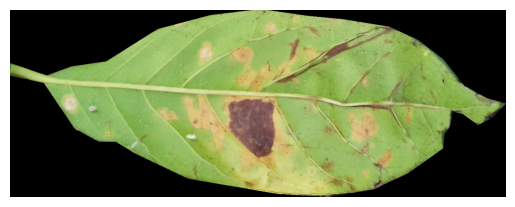
\includegraphics[scale=1]{images/masked_roi_rgb.png}
\caption{Región de interés RGB enmascarada}
\label{img:masked_roi_rgb}
\end{figure}

\begin{figure}[!ht]
\centering
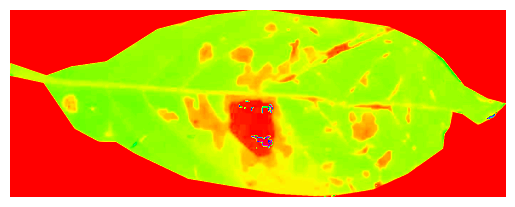
\includegraphics[scale=1]{images/masked_roi_hue.png}
\caption{Región de interés Hue enmascarada}
\label{img:masked_roi_hue}
\end{figure}

Nótese que el valor más bajo para el canal Hue no es un color negro sino un matiz rojo. Esto se debe a la representación circular que emplea el modelo \textsf{HSV}.

\subsection{Histograma de la región de interés}
Una vez que tenemos la región de interés en el canal Hue, procedemos a calcular su histograma (\Cref{code:histogram}) utilizando la máscara (\Cref{img:mask}) de tal manera que no representemos datos fuera del contorno de la hoja. El resultado de la distribución de color puede verse en la \Cref{img:histogram}.

\begin{listing}[!ht]
\inputminted{python}{code_listings/histogram.py}
\caption{Cálcular histograma de la región de interés}
\label{code:histogram}
\end{listing}

\begin{figure}[!ht]
\centering
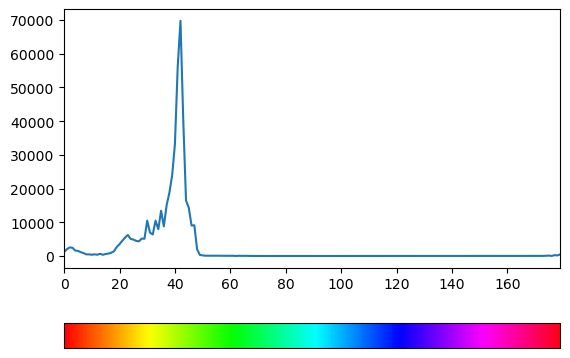
\includegraphics[width=\textwidth]{images/histogram.png}
\caption{Histograma de la región de interés}
\label{img:histogram}
\end{figure}

\subsection{Segmentación de la imagen}
Del histograma nos interesa la región de la hoja que se considera saludable, es decir, la region del espectro Hue en matices verdes, un poco del amarillo-naranja (umbral inferior) y hasta la región azul (umbral superior) para cuando las hojas tengan un verde intenso acercándose a tonos azules.

En el \Cref{code:segmentation} hemos asignado al umbral inferior el valor de 30 y al umbral superior el valor de 120. Segmentamos cada parte de los umbrales y el resultado los unimos usando una operación \texttt{AND} elemento por elemento, resultando en la imagen segmentada apropiadamente (\Cref{img:segmentation}).

\begin{listing}[!ht]
\inputminted{python}{code_listings/segmentation.py}
\caption{Segmentar la región de interés}
\label{code:segmentation}
\end{listing}

\begin{figure}[!ht]
\centering
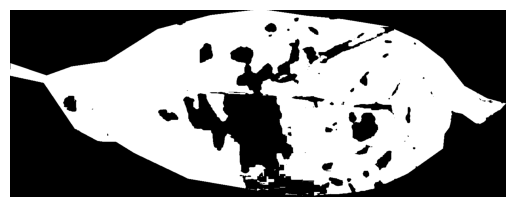
\includegraphics[scale=1]{images/segmentation.png}
\caption{Imagen segmentada}
\label{img:segmentation}
\end{figure}

\subsection{Clasificación de la hoja}
\begin{listing}[!ht]
\inputminted{python}{code_listings/categorize.py}
\caption{Clasificar hoja de café}
\label{code:categorize}
\end{listing}

\section{Presentación de los datos}

\subsection{Resumen}
\begin{listing}[!ht]
\inputminted{python}{code_listings/show_summary.py}
\caption{Mostrar resumen de la clasificación}
\label{code:show_summary}
\end{listing}

\subsection{Imagen original}
\begin{listing}[!ht]
\inputminted{python}{code_listings/show_original_image.py}
\caption{Mostrar imagen original}
\label{code:show_original_image}
\end{listing}

\subsection{Máscara}
\begin{listing}[!ht]
\inputminted{python}{code_listings/show_mask.py}
\caption{Mostrar máscara}
\label{code:show_mask}
\end{listing}

\subsection{Regiones de interés}
\begin{listing}[!ht]
\inputminted{python}{code_listings/show_roi.py}
\caption{Mostrar regiones de interés}
\label{code:show_roi}
\end{listing}

\subsection{Imagen segmentada}
\begin{listing}[!ht]
\inputminted{python}{code_listings/show_segmentation.py}
\caption{Mostrar segmentación de la imagen}
\label{code:show_segmentation}
\end{listing}

\subsection{Histograma}
\begin{listing}[!ht]
\inputminted{python}{code_listings/show_histogram.py}
\caption{Mostrar histograma de la región de interés}
\label{code:show_histogram}
\end{listing}
\chapter{Resultados}
A continuación se presentan los resultados obtenidos durante el procesamiento de las imágenes detallado en el capítulo anterior.

\section{Resultados generales}
La segmentación de la imagen en el canal Hue utilizando los parámetros de umbral inferior y umbral superior (\Cref{sec:segmentation}) con valores de 30 y 120 (\Cref{code:segmentation}), respectivamente, genera los siguientes resultados:

\section{Casos especiales}
\subsection{Iluminación}
\subsection{Envés de la hoja}
\chapter{Conclusiones}

\section{Casos especiales}

\subsection{Iluminación}

\subsection{Envés de la hoja}

\section{Conclusiones específicas}

\section{Conclusiones generales}

\section{Mejoras y trabajo a futuro}
\addcontentsline{toc}{chapter}{Referencias}
\renewcommand{\bibname}{Referencias}
\bibliographystyle{IEEEtran}
\bibliography{References}
\backmatter
\end{document}